% !TeX root = ../../../thesis.tex

\chapter{Custom Current Sampler Schematic}
\label{app:custom-current-sampler-schematic}

In this chapter, the schematic of the current sampler used to measure the current of the 230 V AC can be found in \autoref{fig:custom-current-sampler-schematic}.
The relevant datasheets for parts used can be found in: \cite{lm7824-vr-datasheet}, \cite{lm7805-vr-datasheet}, \cite{lm336z-ref-voltage-datasheet}, \cite{mcp3204-adc-datasheet}, \cite{iso7241m-spi-isolator-datasheet}, \cite{2n7000-n-fet-datasheet} and \cite{sfh617a-optocoupler-datasheet}.


\begin{figure}[htb]
	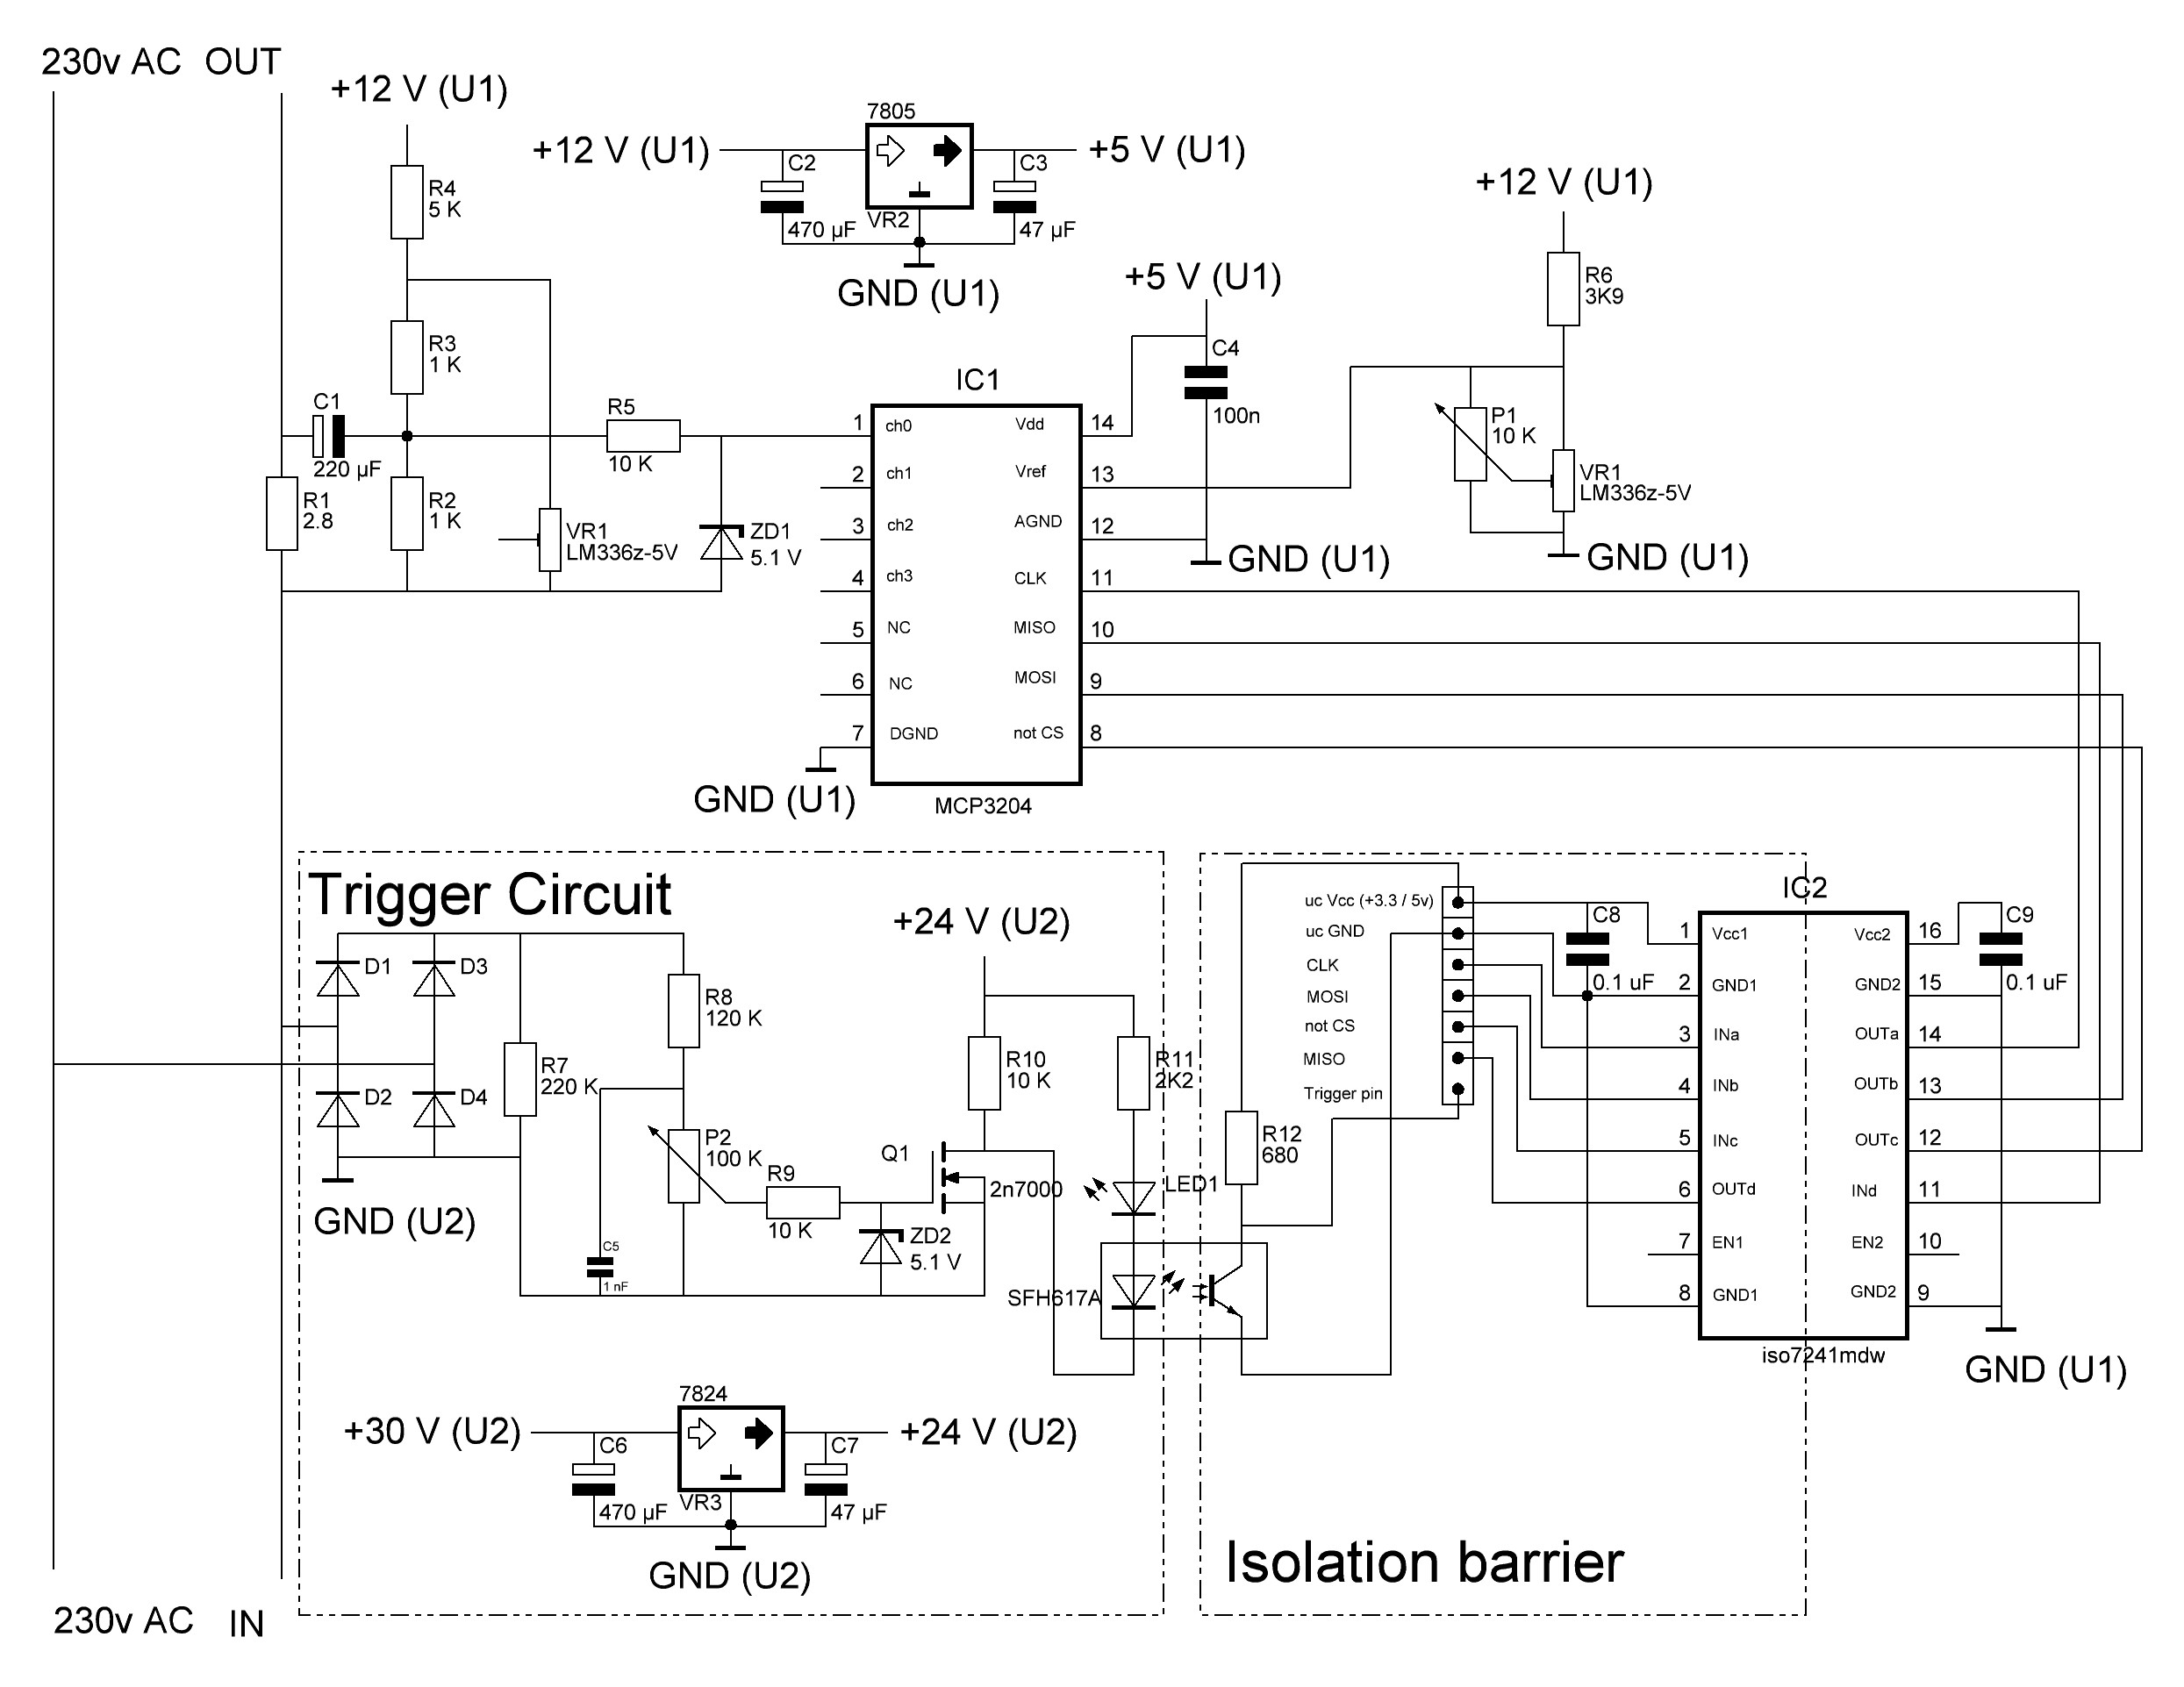
\includegraphics[angle=90,width=\textwidth,height=.9\textheight,keepaspectratio]{chapters/appendix/custom-current-sampler/custom-current-sampler-schematic.jpg}
	\caption{Schematic of the current sampler, with an external ADC which is isolated from the microprocessor and with a triggering circuit.}
	\label{fig:custom-current-sampler-schematic}
\end{figure}
